\documentclass[tikz,border=2pt]{standalone}
\usepackage{amsmath,amssymb}
\usepackage{tikz}

\begin{document}
% In R^n compact means closed and bounded: a closed disc is compact; an open disc is not (its
% rim is missing), nor is an unbounded strip (it runs off to infinity).
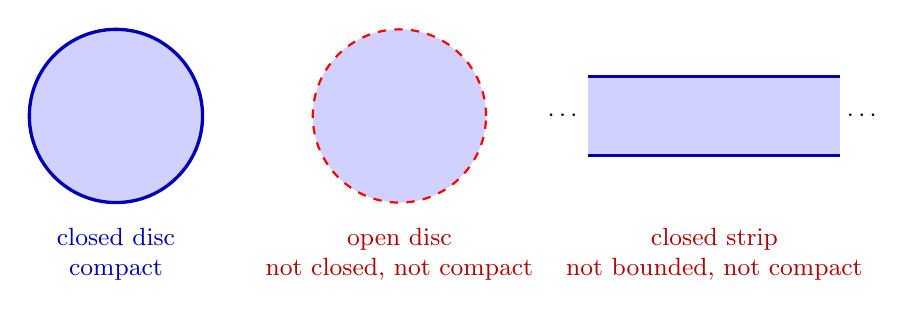
\begin{tikzpicture}[every node/.style={font=\small}]
	\fill[blue!18] (0,0) circle (1.1);
	\draw[blue!70!black, very thick] (0,0) circle (1.1);
	\node[blue!70!black, anchor=north, align=center] at (0,-1.3) {closed disc\\ compact};
	\begin{scope}[xshift=3.6cm]
		\fill[blue!18] (0,0) circle (1.1);
		\draw[red, thick, dashed] (0,0) circle (1.1);
		\node[red!70!black, anchor=north, align=center] at (0,-1.3) {open disc\\ not closed, not compact};
	\end{scope}
	\begin{scope}[xshift=7.6cm]
		\fill[blue!18] (-1.6,-0.5) rectangle (1.6,0.5);
		\draw[blue!70!black, very thick] (-1.6,0.5) -- (1.6,0.5);
		\draw[blue!70!black, very thick] (-1.6,-0.5) -- (1.6,-0.5);
		\node at (1.9,0) {$\cdots$}; \node at (-1.9,0) {$\cdots$};
		\node[red!70!black, anchor=north, align=center] at (0,-1.3) {closed strip\\ not bounded, not compact};
	\end{scope}
\end{tikzpicture}
\end{document}
